\documentclass[crop,border=0pt]{standalone}

\usepackage{mathtools}
\usepackage{tikz}
\usetikzlibrary{positioning,scopes,arrows,shapes,calc}

\begin{document}
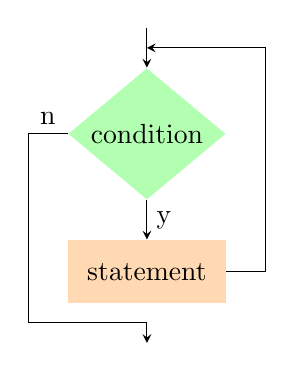
\begin{tikzpicture}[node distance=0,
  process/.style = {rectangle, minimum width=2cm, minimum height=.8cm,
    text centered, fill=orange!30},
  decision/.style = {diamond, minimum width=2cm, minimum height=.8cm,
    text centered, fill=green!30, inner sep=0},
  flow/.style = {draw,->,>=stealth}]

  \node [decision] (cond) {condition};
  \coordinate [above=.5cm of cond] (s0);
  \node [process, below=.5cm of cond] (s1) {statement};
  \coordinate [below=.5cm of s1] (s2);

  \path [flow] (s0) -- coordinate[midway](m) (cond);
  \path [flow] (cond) -- node [right] {y} (s1);
  \path [flow] (s1.east) -- +(.5,0) |- (m);
  \path [flow] (cond.west) -- node [above] {n} +(-.5,0) |- ($(cond)!.9!(s2)$) -| (s2.north);

\end{tikzpicture}
\end{document}
